\section{Model definition}
\label{model-definition}

This Section gives an overview of the models used on the different 
training sets. We first start with the multilayer perceptrons and 
end with the convolutional networks used on the image dataset.

For both models we present the architecture, the initial results 
and the hyperparameter tuning phase.

\subsection{Multilayer perceptron}

The first model used in the experiments is a multilayer perceptron. 
The considered training sets are the ones presented on Subsection 2.2 and 2.3 
namely the first and extended datasets. For the first one, scaled and unscaled 
versions are considered, while for the second the normal and PCA version are tested.

\subsubsection{Network structure}
The starting point for the neural network structure is a 
reasonable network in terms of hidden neurons to prevent over-fitting, 
indeed a high number of units in the hidden layers would end up in learning 
too much from the dataset, leading to poor performances on the test sets.

For this reason, the rule of thumb followed to decide hidden neurons quantity is the 
following: 
$$\#\mathit{hidden\; neurons} = \frac{2}{3}\big(\#\mathit{input\;neurons}
+ \#\mathit{output\;neurons}\big)$$
The next step is to decide the hidden layers number. As using the rule 
presented above gives a quite small amount of units, only two layers are considered,  
indeed, an higher quantity would mean having a real small number of neurons per layer.

Applying this rule ended up in the following architectures on the four 
different training sets, where the output layer is fixed at 10:
\begin{center}
    \begin{tabular}{ |l|r|r|r| } 
        \hline
        Training set & Input & 1st Hidden & 2nd Hidden  \\
        \hline
        132 features unscaled &  132 & 60 & 30 \\
        132 features scaled &  132 & 60 & 30 \\
        180 features scaled &  180 & 80 & 46 \\
        102 features reduced with PCA &  102 & 45 & 30 \\
        \hline
    \end{tabular}
\end{center}

To build the actual model \emph{Tensorflow} and \emph{Keras} libraries 
are used.~\cite{tensorflow}\cite{keras}

\paragraph{Starting point model}
To give reference, Figure \ref{mod} shows the model used on the PCA training set, mentioned at 
the end of Subsection \vref{extended-dataset}, with 
102 input features.
\begin{figure}
    \begin{center}
        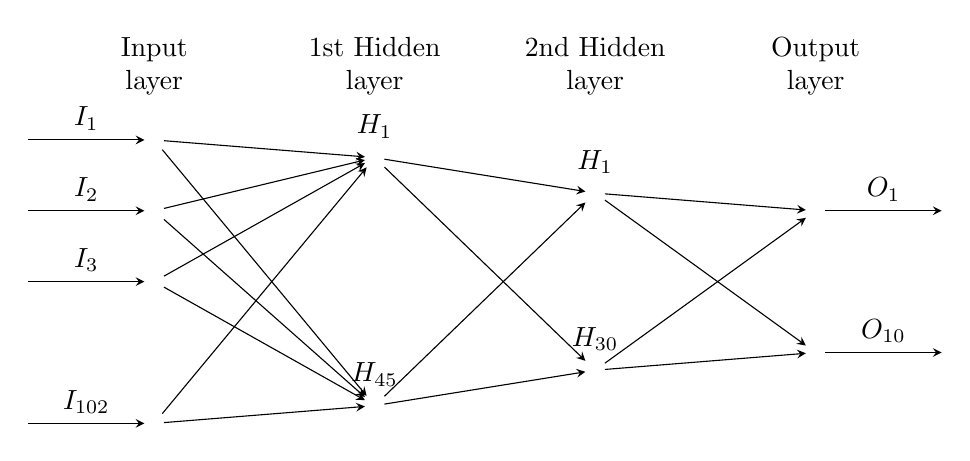
\begin{tikzpicture}[x=1.6cm, y=0.9cm, >=stealth]
            
            % layers
            \foreach \m/\l [count=\y] in {1,2,3,missing,4}
            \node [every neuron/.try, neuron \m/.try] (input-\m) at (0,2.5-\y) {};
            
            \foreach \m [count=\y] in {1,missing,2}
            \node [every neuron/.try, neuron \m/.try ] (hidden-\m) at (1.75,3-\y*1.75) {};
            
            \foreach \m [count=\y] in {1,missing,2}
            \node [every neuron/.try, neuron \m/.try ] (hidden2-\m) at (3.5,2-\y*1.25) {};
            
            \foreach \m [count=\y] in {1,missing,2}
            \node [every neuron/.try, neuron \m/.try ] (output-\m) at (5.25,1.5-\y) {};
            
            %   label
            \foreach \l [count=\i] in {1,2,3,{102}}
            \draw [<-] (input-\i) -- ++(-1,0)
            node [above, midway] {$I_{\l}$};
            
            \foreach \l [count=\i] in {1,45}
            \node [above] at (hidden-\i.north) {$H_{\l}$};
            
            \foreach \l [count=\i] in {1,30}
            \node [above] at (hidden2-\i.north) {$H_{\l}$};
            
            \foreach \l [count=\i] in {1,10}
            \draw [->] (output-\i) -- ++(1,0)
            node [above, midway] {$O_{\l}$};
            
            \foreach \i in {1,...,4}
            \foreach \j in {1,...,2}
            \draw [->] (input-\i) -- (hidden-\j);
            
            \foreach \i in {1,...,2}
            \foreach \j in {1,...,2}
            \draw [->] (hidden-\i) -- (hidden2-\j);
            
            \foreach \i in {1,...,2}
            \foreach \j in {1,...,2}
            \draw [->] (hidden2-\i) -- (output-\j);
            
            \foreach \l [count=\x from 0] in {Input, 1st Hidden, 2nd Hidden, Output}
            \node [align=center, above] at (\x*1.75,2) {\l \\ layer};
        \end{tikzpicture}
    \end{center}
    \caption{MLP architecure used on the PCA dataset}
    \label{mod}
\end{figure}

\paragraph{Activation and loss functions}
The activation function for the input and hidden layers is a \emph{Relu}, 
typically used to prevent the \emph{vanishing gradient problem}, 
and the output one uses a \emph{Softmax} to have classification probabilities
among classes.~\cite{relu}\cite{soft}\cite{vanishing}\\
The loss used is the \emph{Sparse Categorical Crossentropy loss} as it 
is well suited for multiclass classification and, since 
the classes are integers and not one-hot encoded, the sparse version is preferred.~\cite{entropy}

\paragraph{Choosing an optimizer}
When choosing an optimizer for a neural network one must take into account the 
cost of reaching a minimum point on the error function.
Although more complex optimizers exist, build to reduce training 
cost or achieve better performances on deep networks, the one choosen 
for this model is a classic Stochastic Gradient Descent optimizer.

\subsubsection{Training set results}

Section \vref{feature-extraction} talks about the four different 
training sets obtained from the dataset and, without going into details, 
states that there is continuous improvement. 
We now give a more detailed look on training performances, after 
detailing how class imbalance is faced and the applied validation method.

Note that all the random seeds used by Tensorflow are fixed 
to make results reproducible. This step is necessary as many parameters initial 
value is random, for instance, the neural network weights.

\paragraph{Class imbalance}
To deal with the minority of some classes, balancing techniques should be 
applied when fitting the model. One of the possible approaches, and the one followed
here, is to assign class weights. 

The main idea is to penalize errors made on not well represented classes to account 
for their minority, in particular, each class has weight:
$$w_i = \frac{\#\mathit{total\;samples}}{\#\mathit{classes} * \#\mathit{samples\;of\;class\;i}}$$

Class weights computation relies on the \emph{compute class weights} function with the balanced logic
from sklearn.~\cite{classweight}\\
The following are the computed quantities for the dataset classes:
\begin{center}
    \begin{tabular}{ |l|c|c| } 
        \hline
        Class name & Number of samples & Class weight \\
        \hline
        air conditioner & 500 & 0.8998 \\
        car horn & 208 & 2.1629 \\
        children playing & 500 & 0.8998 \\
        dog bark & 500 & 0.8998 \\
        drilling & 500 & 0.8998 \\
        engine idling & 517 & 0.8702 \\
        gun shot & 190 & 2.3678 \\
        jackhammer & 548 & 0.8209 \\
        siren & 536 & 0.8393 \\
        street music & 500 & 0.8998 \\
        \hline
    \end{tabular}
\end{center}
As expected, the less numerous classes have higher class weight than the rest,
in particular, the misclassification of a car horn sample
counts more than double than an air conditioner one.

\paragraph{Stratified cross-validation}
To estimate performance on the training set, stratified cross-validation with 
five folds is used. Basically the dataset is divided into five parts 
and a model is repeatedly trained on four and tested on one, all while considering class 
distribution, indeed, the original distribution of the classes is maintained 
in the splits.~\cite{stratified}

The stratified approach is required as there is class imbalance on the training set.
In fact, applying a classical cross-validation could show misleading results, 
for instance when the minority classes are more present 
in the test fold rather than the training ones; in such cases the loss would be 
higher.
The mean accuracy on the test folds gives a hint about the model performance.

For this step the \emph{Stratified KFold} class from scikit learn is used.~\cite{cross-scikit}

\paragraph{Results}
The following are the results on the training sets, using the architectures 
presented at the beginning of the Subsection. 

The runs are performed with a five fold stratified cross-validation. 
At each fit, epochs are fixed at 100, 
batch size is set at 64 and class weights, computed once on 
the entire training set, are considered. 
The optimizer is the stochastic gradient descent with zero momentum and 
0.01 learning rate. 

Mean accuracy and standard deviation are computed on the 
folds results.
\begin{center}
    \begin{tabular}{ |l|r|r| } 
        \hline
        Training set & Mean accuracy & St. deviation \\
        \hline
        132 features unscaled &  0.1138 & 0.0039 \\
        132 features scaled &  0.5743 & 0.0324 \\
        180 features scaled &  0.6363 & 0.0494 \\
        102 features reduced with PCA &  0.6188 & 0.0420 \\
        \hline
    \end{tabular}
\end{center}

There is a great improvement after scaling the training set, after 
that small refinements are made.
As accuracy is the best on the last two training sets, those are the two selected to 
perform the hyperparameter tuning.

\subsubsection{Hyperparameter tuning}

The last two tries with feature extraction lead to the best results 
with stratified cross-validation. Although the two models are reasonable, 
they can not be the final ones as many parameters are left on their default value, 
for instance, learning rate and momentum of the optimizer are untouched. 

The main goal now is to experiments with ranges of model parameters 
to find a better one. From now on, the model build on the 180 features training set is 
called \emph{Extended model}, 
while the one tested on the PCA training set is named \emph{PCA model}.

\paragraph{Grid and random search comparison}
Two of the most commonly used strategies in hyperparameter optimization
are \emph{grid} and \emph{random search}~\cite{random-grid}. 

In both cases we define ranges of parameters to test different combinations, 
for instance, fixed the number of neurons, one could try to find the best 
combination of learning rate and momentum that optimize accuracy on the training set.

While similar, the two methodologies differs in the amount of exploration they do.
The grid search try all the possible combinations of parameters, while the 
random approach fixes a number of iterations and picks an arbitrary unseen 
combination each time. 

Obviously the first one is more computationally expensive than the second, if 
we fix a small amount of possible iterations, but in theory it finds a better result
than going the random route. 
Nonetheless the grid search can led to over-fitting and in practice random 
search in preferred.

\paragraph{Random search}
We now run a random search with various parameters 
to optimize the initial models.
Note that class weights are still considered and the models are evaluated
again with a five fold stratified cross-validation.
The optimizer used is the stochastic gradient descent.

The considered ranges for parameters for this run are: 
\begin{enumerate}
    \item \emph{Neurons}: input layer has dimension $I$, last layer is fixed at 10, while 
    the two hidden layers are tested with a number of neurons respectively 
    equals to: 
    $$H_1 + 2i\;\;\text{and}\;\;H_2 + 2j,\;\;\text{with}\;\; i, j \in \{-2,-1,0,1,2\}$$
    \item \emph{Learning rate}: $0.001, 0.01, 0.1, 0.5$;
    \item \emph{Momentum}: $0.0, 0.01, 0.1, 1$;
    \item \emph{Epochs}: $60, 80, 100$;
    \item \emph{Batch size}: $32, 64$.
\end{enumerate}

The quantities $I$, $H_1$, $H_2$, which are input, first hidden and second hidden 
layer dimensions, depend on the initial network architecture.
As stated before, the two models considered are the following: 
\begin{center}
    \begin{tabular}{ |l|r|r|r|} 
        \hline
        Model name & $I$ & $H_1$ & $H_2$ \\
        \hline
        Extended model & 180 & 80 & 46 \\
        PCA model & 102 & 45 & 30 \\
        \hline
    \end{tabular}
\end{center}

An \emph{early stopper} with patience equals to three is used on the training to stop it when no progress is made with 
respect to the last three epochs result.~\cite{early}
The search is performed with 100 iterations for both rounds.

The Extended model is trained on the 180 features dataset, 
while the PCA model on the 102 features dataset.

\paragraph{Final models}
The first round of the random search, performed on the Extended model, finds 
in the following parameters:
\begin{itemize}
    \item Neurons: 180 for input, 76 for the first hidden layer, 50 for the second and 10 for output;
    \item Momentum: 0.01
    \item Learning rate: 0.01
    \item Epochs: 80
    \item Batch size: 64
\end{itemize}
We can see an improvement in accuracy by comparing it to the starting point model:
\begin{center}
    \begin{tabular}{ |l|r|r| } 
        \hline
        Model & Mean accuracy & St. deviation \\
        \hline
        Initial extended model & 0.6363 & 0.0494\\
        Tuned extended model & 0.6497 & 0.0431\\
        \hline
    \end{tabular}
\end{center}

The second random search on the smaller PCA model, finds these parameters:
\begin{itemize}
    \item Neurons: 102 for input, 45 for the first hidden layer, 32 for the second and 10 for output;
    \item Momentum: 0.01
    \item Learning rate: 0.1
    \item Epochs: 80
    \item Batch size: 32
\end{itemize}
As before, comparing it with the starting model, we can see some better results:
\begin{center}
    \begin{tabular}{ |l|r|r| } 
        \hline
        Model & Mean accuracy & St. deviation \\
        \hline
        Initial PCA model & 0.6188 & 0.0420\\
        Tuned PCA model & 0.6270 & 0.0315\\
        \hline
    \end{tabular}
\end{center}

\paragraph{Final remarks on MLP}
Unexpectedly PCA application lead to worse results compared to the 180
feature dataset. Even after the random search, the so called Tuned Extended model
performs better. For this reason this is the final multilayer perceptron
evaluated on the test set.

\subsection{Convolutional neural network}
This subsection presents the results obtained by a convolutional
neural network trained on the image datasets presented at the end of 
Section \vref*{feature-extraction}.
We start by giving an overview of the network, to then proceed 
with the training results and hyperparameter tuning.

\subsubsection{Network structure}
The structure of a neural network for image classification 
consists of convolutional layers followed by pooling layers, 
and, at the end, densely connected ones to have the output classification.

The main idea is to extract relevant features from the images 
with the convolutional layers, that apply a kernel to the input 
to detect patterns and image features.
After the convolution part there is a pooling layer that reduces dimensionality.
At the end, densely connected layers classify the obtained features.

\paragraph{Stacking convolutions}
Taking inspiration from the \emph{VGG19 architecture}, that stacks two or more 
convolutional layers to then apply pooling, the network is built with 
the following layers:~\cite{vgg}
\begin{itemize}
    \item \emph{Two Convolution layers}: each one with 8 filters, kernel size of $5 \times 5$, Relu activation, $1 \times 1$ stride;
    \item \emph{MaxPooling}: pooling size of $2 \times 2$, $3 \times 3$ strides;
    \item \emph{Two Convolution layers}: each one with 16 filters, kernel size of $3 \times 3$, Relu activation, $1 \times 1$ stride;
    \item \emph{MaxPooling}: pooling size of $2 \times 2$, $3 \times 3$ strides;
    \item \emph{Flatten layer};
    \item \emph{Dense layers}: dimensions are 2000, 800, 200 and 60, Relu activation;
    \item \emph{Output}: 10 neurons and softmax activation.
\end{itemize}

\begin{figure}[h]
    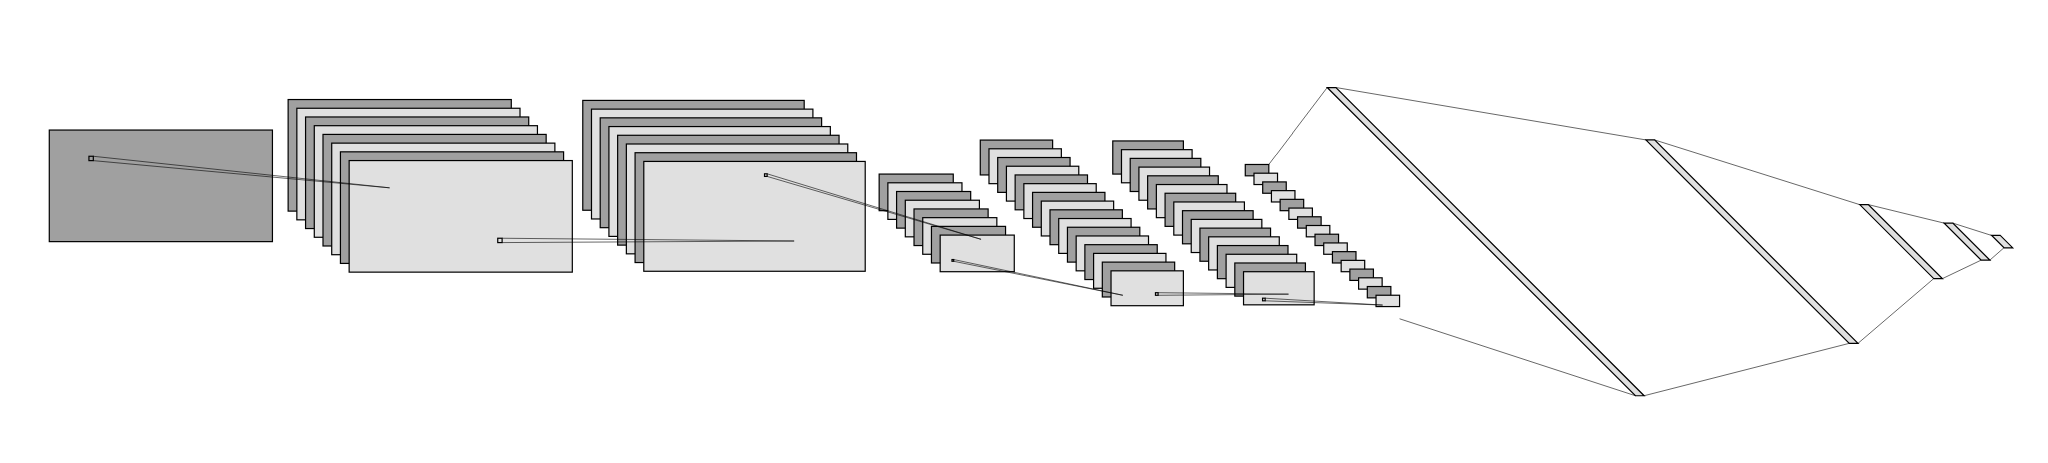
\includegraphics[width=\textwidth]{images/cnn.png}  
    \caption{Diagram of the network used in the experiments. We can see 
    the first two convolutions, followed by the max pooling layer, first two blue layers and 
    the red one respectively. After that, two other convolutions and 
    another max pooling, and finally the densely connected ones, in gray. We can see the principle of 
    learning higher level features and fine grain ones, indeed the dimensionality increases 
    from the first convolutions to the seconds.}  
    \label{cnn}
\end{figure}

\paragraph{Kernel sizes, filters and strides}
Two crucial parameters for a convolutional layers are the number of filters, 
the kernel size and strides dimensions. 
The filter number represent the number of ways a 
convolutional layer sees the image, while the kernel size makes the area 
considered by the layer bigger or smaller. One can see a small kernel size as a way 
of learning fine grain features, on the opposite, a bigger size capture higher level image characteristics.
Finally, strides determine the reduction on the output shape, for instance, a stride equals to 
two, reduces the output shape in half.

One important factor in choosing the values for this parameters is the output dimensionality, 
in fact, while strides reduces it, higher filters and smaller kernels increase 
the feature space.

For this reasons, filters number is smaller and kernel size is bigger for the first 
convolutional layers, while we have more filters and smaller kernel for the consequent ones.
The idea is to learn higher level features first, to then capture small peculiarities.
For the first architecture stride on convolutional layers is kept at one, later, an higher value is tested.

\subsubsection{Training set results}
We now present the results on the image dataset using the model introduced in 
the \emph{Stacking convolutions} paragraph. Stratified 
cross validation with five folds is once again used, the number of epochs 
is fixed at 10 and we use an early stopper with patience equals to two, to stop training 
if no improvement is made on accuracy for two epochs. The principle of 
class weights, introduced with the previous MLP experiments, is reused this time.
The optimizer is the Adam one, as it is built to speed up training on 
deep neural networks, with learning rate set to 0.001.

We can compare results with previously tuned multilayer perceptrons, as the validation
technique is the same.
\begin{center}
    \begin{tabular}{ |l|r|r| } 
        \hline
        Model & Mean accuracy & St. deviation \\
        \hline
        Tuned extended model& 0.6497 & 0.0431 \\
        Tuned PCA model & 0.6270 & 0.0315 \\
        Initial CNN & 0.5383 & 0.0395 \\
        \hline
    \end{tabular}
\end{center}
Results with the CNN are a big downgrade from previously tested models, 
but we need to consider the fact that those have their 
hyperparameters tuned.

\subsubsection{Hyperparameter tuning}
Training a CNN is really expensive compared to the MLP networks.
Performing a full random search is infeasible with the resources we have, therefore, 
to have an idea about the impact on accuracy of the network parameters, we run 
cross-validation on the following models, that, for simplicity, have a name.
\begin{center}
    \begin{tabular}{ |c|r|r|r|l| } 
        \hline
        Name & Filters & C. strides & P. strides & Dense structure \\
        \hline
        $C_0$ & 8 &  $1 \times 1$ & $3 \times 3$ & 2000, 800, 200, 60 \\
        $C_1$ & 8 &  $2 \times 2$ & $2 \times 2$ & 300, 150, 80, 25 \\
        $C_2$ & 16 & $1 \times 1$ & $3 \times 3$ & 5000, 2000, 800, 200, 60 \\
        $C_2$ & 16 & $2 \times 2$ & $2 \times 2$ & 600, 200, 80, 25 \\
        \hline
    \end{tabular}
\end{center}

The filter quantity represent the number of filters for the first convolutions. 
The subsequent ones have double that quantity.
Kernel size is fixed at $5 \times 5$ and $3 \times 3$ for the first two and last 
two convolutional layers respectively. 

The \emph{C. strides} values are the strides for convolutions, a value of one does not 
reduce dimensionality, while a value of three reduces the output dimensionality by an  half.\\
The \emph{P. strides} are the pooling layers strides. As before, two reduces dimensionality 
by an half and three by two thirds.\\
Lastly, the \emph{dense structure} sums up the last layers architecture. For instance, 
the model $C_1$ have four consequent densely connected layers, with 300, 150, 80 and 
25 neurons respectively, followed by a final output layer of 10 neurons.

A different learning rate is also tested for the Adam optimizer, 
indeed 0.001 and 0.003 runs are performed.
The rest of the network is the same as the initial CNN, thus activation is always a Relu, 
apart from the Softmax on the output layer and pooling size is fixed at $2 \times 2$.

Note that $C_0$ is the same as the initial model, but we retest it with another learning rate.

\paragraph{Cross-validation results}
The following are cross-validation results. 
The settings for the cross validation are the same ones presented in the \emph{Training set results}
Subsubsection, apart from the epochs that this time are increased to 15 and the Adam 
learning rate that is now variable.

We can see that the $C_3$ model is the best performer, even if the differences among models are not really big.
\begin{center}
    \begin{tabular}{ |c|r|r|r|r| } 
        \hline
        \multirow{2}{*}{Model name} & \multicolumn{2}{c|}{0.001 l.r.} & \multicolumn{2}{c|}{0.003 l.r.}  \\
        \cline{2-5}
        & M. accuracy & St. deviation & M. accuracy & St. deviation \\
        \hline
        $C_0$ & 0.5383 & 0.0395 & 0.5150 & 0.0253 \\
        $C_1$ & 0.5347 & 0.0480 & 0.5223 & 0.0480 \\
        $C_2$ & 0.5285 & 0.0325 & 0.3909 & 0.1455 \\
        $C_3$ & 0.5412 & 0.0474 & 0.5341 & 0.0451 \\
        \hline
    \end{tabular}
\end{center}

The table shows that increasing the learning rate always leads to worse results.
The best model found, and the one that is measured on the test set is 
the $C_3$ architecture with 0.001 learning rate for the Adam optimizer.

\paragraph{Overfitting and underfitting}
Cross-validation results gives an hint about overfitting and underfitting. Indeed, 
by looking at the trainable parameters quantity using Keras summary function we have the following results.
\begin{center}
    \begin{tabular}{ |c|r| } 
        \hline
        Model name & Trainable parameters\\
        \hline
        $C_0$ & 13011950 \\
        $C_1$ & 256095 \\
        $C_2$ & 67957294 \\
        $C_3$ & 923789 \\
        \hline
    \end{tabular}
\end{center}
The numbers might indicate that the $C_1$ model is underfitting, as the number 
of parameters does not create the required complexity in the model to capture the dataset, 
the $C_2$ and initial models are overfitting, as they have too many parameters 
thus they are learning too much from the training. 
$C_3$ seems to be at a sweet spot between the two, confirmed by the higher accuracy.

\paragraph{Final remarks on CNN}
Unfortunately, the high cost of training a CNN made impossibile to run a Random search 
starting from the initial network structure, nonetheless a total 
of eight models are tested. Results are worse than the ones obtained 
with the MLP models. 
\newpage